\documentclass[11pt,a4paper]{article}
\usepackage[T1]{fontenc}
\usepackage[margin=2.3cm]{geometry}
\usepackage{amsmath,amssymb}
\usepackage{graphicx}
\usepackage[dvipsnames]{xcolor}
\usepackage{enumitem}
\usepackage[colorlinks=true,linkcolor=blue,urlcolor=blue]{hyperref}
\setlength{\parskip}{0.6em}
\setlength{\parindent}{0pt}
\begin{document}

\begin{center}{\LARGE\bfseries openpinn}\\[0.4em]{\large Teach a network the heat equation, then make it find the physics, in three sessions.}\\[0.2em]\small PAN IIT OSS explainer \textbullet{} higher secondary to advanced undergraduate (levels 4-6)\end{center}

\section*{Why this exists}
A differential equation says how a quantity changes. A physics-informed network is trained so that a flexible curve obeys that equation as well as the data. This explainer shows, with only numpy and the chain rule, how such a network is built, checked and used.

\section*{The end goal}
Solve the heat equation with a physics-informed network. The end goal is to solve the heat equation with a physics-informed network and to use it backwards to recover an unknown diffusivity from noisy readings. The same idea is used for fluids, structures and materials when measurements are sparse; for easy forward problems classical solvers remain faster.

\section*{How the three sessions build up}
\begin{enumerate}[nosep]
\item \textbf{Session 1: A flexible curve that can also obey a law} (Level 1, conceptual interactive model, 60 min).
\item \textbf{Session 2: Train a tiny network on a differential equation} (Level 2, mathematical engineering model, 75 min).
\item \textbf{Session 3: A network that solves the heat equation, and finds its diffusivity} (Level 3, simulation and validation, 90 min).
\end{enumerate}

\section{Session 1: A flexible curve that can also obey a law}

\subsection*{A. Real-world problem}
A cup of tea is measured six times in its first minute and the readings are noisy. You must predict the temperature excess over room temperature for the whole next minute too. A flexible curve can pass near all six readings and still swing wildly where there are no readings. But you also know a law: the excess falls at a rate proportional to itself. In scaled units the law reads u' = -u, where u' is the slope of the curve. This is the idea behind physics-informed networks: the curve is bent by the data and also by the law. (General education only: this is a toy model, not a design tool.)

\subsection*{B. Concept and theory}
A neural-network unit is a smooth step, tanh(s), which is -1 far to the left, +1 far to the right and 0 at s = 0. Moving it with x - m and sharpening it with a steepness gives a bump. A curve built from H bumps is u(x) = c\_1 tanh(3 (x - m\_1)) + ... + c\_H tanh(3 (x - m\_H)) + c\_0. In this session the centres m\_j are fixed, evenly spread over 0 to 2, and only the weights c are chosen. Least squares chooses the weights that make the sum of (curve - reading)\textasciicircum{}2 smallest; a tiny penalty on the size of the weights keeps the sums sensible. The slope of the curve is again a weighted sum, since the slope of tanh(s) is 1 - tanh(s)\textasciicircum{}2. So the statement 'slope + value = 0 at chosen points' is also a set of linear equations in the weights. We add them to the fit with a strength lam: this is a physics-informed fit.

\begin{itemize}[nosep]
\item x: time (scaled) (dimensionless)
\item u(x): temperature excess (scaled) (dimensionless)
\item H: number of tanh bumps (units) (count)
\item c\_j: weight of bump j (dimensionless)
\item m\_j: centre of bump j (same unit as x)
\item lam: strength of the law compared with the data (dimensionless)
\end{itemize}

\begin{equation*}
u(x)=c_0+\sum_{j=1}^{H} c_j\tanh\!\big(3\,(x-m_j)\big)
\end{equation*}

\begin{equation*}
u'(x)=\sum_{j=1}^{H} 3\,c_j\left(1-\tanh^2\!\big(3\,(x-m_j)\big)\right)
\end{equation*}

\begin{equation*}
\min_c\ \sum_{i=1}^{6}\big(u(x_i)-y_i\big)^2+\lambda\sum_{k=1}^{21}\big(u'(s_k)+u(s_k)\big)^2
\end{equation*}

\begin{center}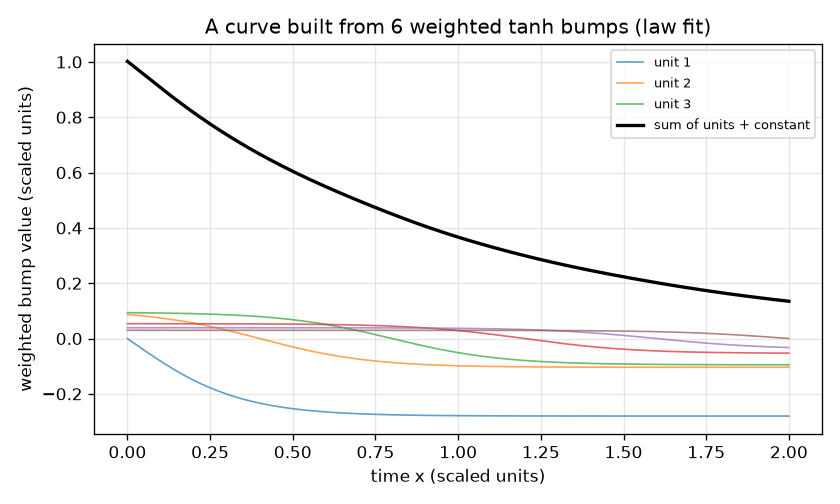
\includegraphics[width=0.85\linewidth]{figures/s01_bumps_sum.png}\\\small A curve is a sum of weighted tanh bumps plus a constant.\end{center}

\subsection*{E. Worked example}
Fit 12 bumps to the six readings, first with the data only and then with the law (lam = 1). Compare the rms error against exp(-x) over x from 0 to 2, and the largest value of \textbar{}u' + u\textbar{}.
\begin{enumerate}[nosep]
\item The readings are y = exp(-x) + noise at x = 0, 0.2, ..., 1.0. For example at x = 0.4 the reading is exp(-0.4) + 0.025 = 0.6703 + 0.025 = 0.695.
\item Data only: 13 weights (12 bumps and the constant) must fit 6 numbers, so many curves fit equally well; the fit passes within 0.05 of every reading but its rms error against exp(-x) over 0 to 2 is above 0.5.
\item With the law (21 law rows on 0 to 2, lam = 1): the rms error drops below 0.001.
\item The largest \textbar{}u' + u\textbar{} is above 2 without the law and below 0.03 with it: the law-fit curve nearly obeys the equation everywhere, not only at the dots.
\end{enumerate}
\textbf{Answer.} Readings only: rms error above 0.5. Readings plus law: rms error below 0.001, and the largest \textbar{}u' + u\textbar{} falls from above 2 to below 0.03.

\subsection*{F. Questions}
\begin{enumerate}[nosep]
\item \textbf{Conceptual.} Why can a curve that passes within 0.05 of all six readings still be a poor prediction for the second minute?
\item \textbf{Numerical.} A candidate curve is u = exp(-0.9 x). Compute the law residual u' + u at x = 1. Is the candidate a solution of u' = -u?
\item \textbf{Graph and simulation interpretation.} In the app, with 6 units, compare the red and green curves at x = 2. What does the difference tell you, and what is the error with the law on?
\item \textbf{Design and optimisation challenge.} Design: you can afford 6 units at most and want the rms error below 0.01. Choose the law weight, and say what happens if it is too large or if you use only 3 units.
\end{enumerate}

\section{Session 2: Train a tiny network on a differential equation}

\subsection*{A. Real-world problem}
Hot tea cools so that its excess temperature u obeys du/dx = -u, with u(0) = 1 (scaled units; x is time). The exact answer is exp(-x). Instead of stepping the equation forward in time, we ask a network to be a function whose slope plus value is zero at chosen points (collocation points) and which equals 1 at x = 0. How many collocation points must we choose before the network is right everywhere, not only at the points?

\subsection*{B. Concept and theory}
A network with H tanh units computes u(x) = sum\_j c\_j tanh(a\_j x + d\_j) + e. Its slope follows from the chain rule: since d tanh(z)/dz = 1 - tanh(z)\textasciicircum{}2 =: s, the slope is du/dx = sum\_j c\_j a\_j s\_j. A loss L measures how bad the network is; backpropagation uses the chain rule to find how L changes with each parameter, so each parameter can be nudged downhill. Adam is a gradient method that keeps running averages of the gradient and of its square, so parameters with small gradients still move. For the equation we do not need data: the loss is the average of the squared residual (du/dx + u) at N collocation points plus the squared boundary error (u(0) - 1)\textasciicircum{}2. The residual term is zero exactly when the law holds at the points; the boundary term fixes the amplitude, since the law alone allows any multiple of exp(-x). Between the points the law is not enforced: more points means a smaller gap.

\begin{itemize}[nosep]
\item a\_j, d\_j: input weight and shift of unit j (dimensionless)
\item c\_j, e: output weight of unit j and constant offset (dimensionless)
\item s\_j: slope of tanh at unit j: 1 - tanh\textasciicircum{}2 (dimensionless)
\item N: number of collocation points on x = 0 to 2 (count)
\item r(x): residual du/dx + u (dimensionless (scaled))
\item L: loss: mean squared residual plus boundary error squared (dimensionless)
\end{itemize}

\begin{equation*}
u(x)=\sum_{j=1}^{H} c_j\tanh(a_j x+d_j)+e,\qquad \frac{du}{dx}=\sum_{j=1}^{H} c_j a_j\left(1-\tanh^2(a_j x+d_j)\right)
\end{equation*}

\begin{equation*}
\frac{\partial u}{\partial c_j}=\tanh_j,\quad \frac{\partial u}{\partial a_j}=c_j s_j\,x,\quad \frac{\partial u}{\partial d_j}=c_j s_j,\quad s_j=1-\tanh_j^2
\end{equation*}

\begin{equation*}
\mathcal L=\frac1N\sum_{i=1}^{N}\left(\frac{du}{dx}(x_i)+u(x_i)\right)^2+\big(u(0)-1\big)^2
\end{equation*}

\begin{equation*}
m\leftarrow 0.9\,m+0.1\,g,\quad v\leftarrow 0.999\,v+0.001\,g^2,\quad p\leftarrow p-\eta\,\frac{\hat m}{\sqrt{\hat v}+10^{-8}}
\end{equation*}

\begin{center}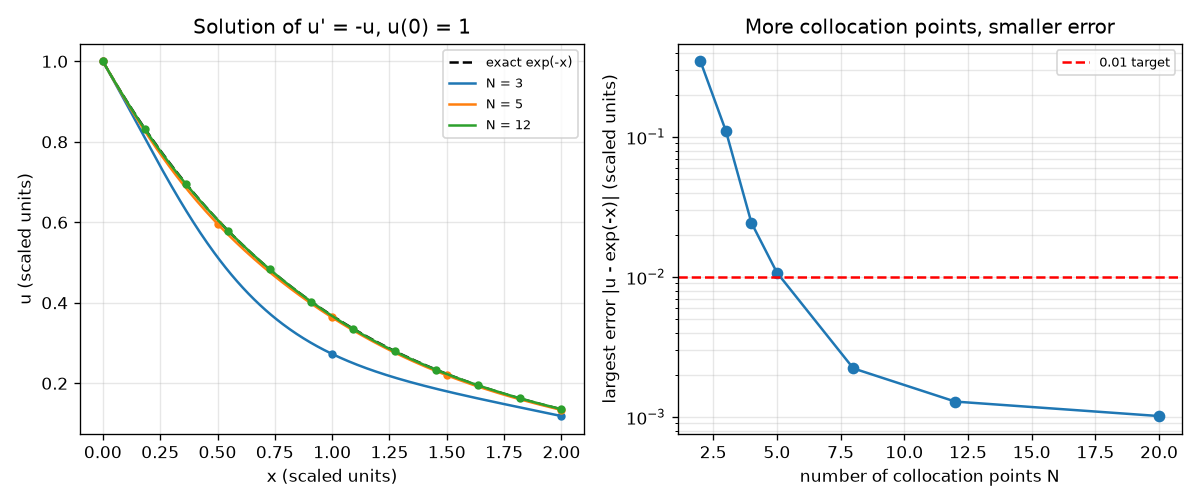
\includegraphics[width=0.85\linewidth]{figures/s02_collocation.png}\\\small Left: the network solution for N = 3, 5, 12 against exp(-x). Right: largest error against the number of collocation points.\end{center}

\subsection*{E. Worked example}
A trial solution u = exp(-0.8 x) is tested at the three collocation points x = 0, 1, 2. Compute the loss of Section B and compare with the exact solution; then read the error table for N collocation points.
\begin{enumerate}[nosep]
\item u = exp(-0.8 x) has slope -0.8 exp(-0.8 x), so the residual is u' + u = 0.2 exp(-0.8 x).
\item At x = 0, 1, 2 the residuals are 0.2, 0.2 exp(-0.8) = 0.0899 and 0.2 exp(-1.6) = 0.0404.
\item Mean of the squares = (0.04 + 0.00808 + 0.00163) / 3 = 0.01657. The boundary term is (u(0) - 1)\textasciicircum{}2 = 0, so the loss is 0.0166.
\item For the exact solution exp(-x) every residual is 0 and the loss is 0.
\item Training the network (10 units) for several N gives the largest error against exp(-x) on 0 to 2: above 0.3 for N = 2, between 0.01 and 0.02 for N = 5, below 0.01 for N = 8 and below 0.002 for N = 20.
\end{enumerate}
\textbf{Answer.} The trial solution has loss 0.0166 (the exact solution 0). The network error falls from above 0.3 at N = 2 to below 0.01 at N = 8.

\subsection*{F. Questions}
\begin{enumerate}[nosep]
\item \textbf{Conceptual.} Why does the loss need the boundary term (u(0) - 1)\textasciicircum{}2? What would the network do without it?
\item \textbf{Numerical.} For a single unit u = tanh(x) (c = 1, a = 1, d = 0, e = 0), compute the residual u' + u at x = 0.5.
\item \textbf{Graph and simulation interpretation.} In the error-against-N plot, what is the smallest N tested that brings the largest error below 0.01, and what happens at N = 2?
\item \textbf{Design and optimisation challenge.} Design: you can afford at most 8 collocation points (each costs a training evaluation) but need the largest error below 0.01 on 0 to 2. Is that possible, and what would you change if a colleague wanted 0.001?
\end{enumerate}

\section{Session 3: A network that solves the heat equation, and finds its diffusivity}

\subsection*{A. Real-world problem}
A thin metal rod of length 1 (scaled units) has both ends held at temperature 0 and starts with a smooth hump of heat, u(x, 0) = sin(pi x). Heat leaks out and the rod cools according to the heat equation u\_t = alpha u\_xx, where alpha is the diffusivity. We ask a network u(x, t) to satisfy the equation inside, the ends and the starting hump, and we judge it against the exact solution and against a classical solver. Then we turn the problem around: from 30 noisy thermometer readings, what is alpha? (A simplified teaching model: real rods lose heat from their sides, and diffusivity varies with temperature.)

\subsection*{B. Concept and theory}
The heat equation u\_t = alpha u\_xx on 0 \textless{}= x \textless{}= 1 with u(0, t) = u(1, t) = 0 and u(x, 0) = sin(pi x) has the exact solution u = sin(pi x) exp(-alpha pi\textasciicircum{}2 t): the hump keeps its shape and decays, with half-life ln 2 / (alpha pi\textasciicircum{}2). The network u(x, t) = sum\_j c\_j tanh(a\_j x + b\_j t + d\_j) + e has, by the chain rule, u\_t = sum c\_j b\_j s\_j and u\_xx = sum c\_j a\_j\textasciicircum{}2 s2\_j, where s = 1 - tanh\textasciicircum{}2, s2 = -2 tanh s and s3 = s (6 tanh\textasciicircum{}2 - 2) are the first three derivatives of tanh. Backpropagation through these formulas needs s3 too. The key correctness check compares the formulas with finite differences of u. The loss is w\_res times the mean squared residual (u\_t - alpha u\_xx) at N random interior points, plus the mean squared boundary error, plus the mean squared initial error. The classical reference is the explicit scheme: each interior value moves towards the average of its neighbours, u\_i(new) = u\_i + r (u\_(i-1) - 2 u\_i + u\_(i+1)) with r = alpha dt / dx\textasciicircum{}2, which is stable only for r \textless{}= 1/2. For the inverse problem alpha becomes a trainable parameter, a data term compares the network with the noisy readings, and a classical alternative is to fit alpha directly when the form of the solution is known.

\begin{itemize}[nosep]
\item x: position along the rod (scaled) (dimensionless)
\item t: time (scaled) (dimensionless)
\item u(x, t): temperature (scaled) (dimensionless)
\item alpha: diffusivity (true value 0.1) (scaled length\textasciicircum{}2 per time)
\item w\_res: weight of the residual term in the loss (dimensionless)
\item N: number of collocation points (count)
\item r: explicit-scheme number alpha dt / dx\textasciicircum{}2 (dimensionless)
\end{itemize}

\begin{equation*}
u_t=\alpha\,u_{xx},\qquad u(0,t)=u(1,t)=0,\qquad u(x,0)=\sin(\pi x)
\end{equation*}

\begin{equation*}
u(x,t)=\sin(\pi x)\,e^{-\alpha\pi^2 t},\qquad t_{1/2}=\frac{\ln 2}{\alpha\pi^2}
\end{equation*}

\begin{equation*}
u=\sum_j c_j\tanh z_j+e,\quad u_t=\sum_j c_j b_j\,s_j,\quad u_{xx}=\sum_j c_j a_j^2\,s_j'',\quad z_j=a_jx+b_jt+d_j
\end{equation*}

\begin{equation*}
\mathcal L=w_{\mathrm{res}}\,\overline{(u_t-\alpha u_{xx})^2}+\overline{u(0,t)^2}+\overline{u(1,t)^2}+\overline{(u(x,0)-\sin\pi x)^2}
\end{equation*}

\begin{equation*}
u_i^{n+1}=u_i^n+r\,(u_{i-1}^n-2u_i^n+u_{i+1}^n),\qquad r=\frac{\alpha\,\Delta t}{\Delta x^2}\le\frac12
\end{equation*}

\begin{equation*}
E=\frac{\lVert u_{\mathrm{net}}-u_{\mathrm{exact}}\rVert_2}{\lVert u_{\mathrm{exact}}\rVert_2}
\end{equation*}

\begin{center}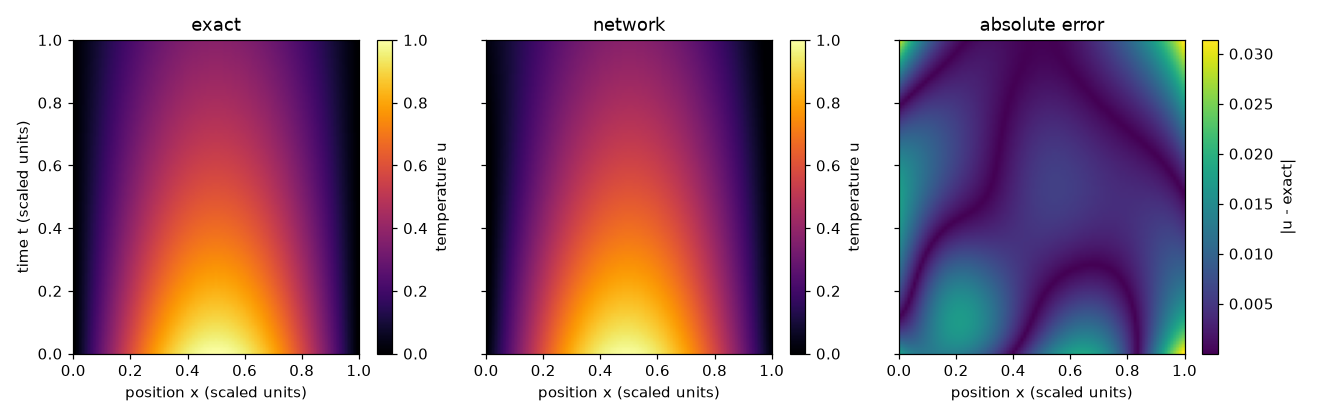
\includegraphics[width=0.85\linewidth]{figures/s03_heatmaps.png}\\\small Exact solution, network solution and absolute error of the heat equation on x, t in [0, 1].\end{center}

\subsection*{E. Worked example}
For alpha = 0.1 find the exact temperature at the rod centre at t = 1 and the half-life, then compare the trained network and the finite-difference scheme (20 intervals, r = 0.4) with it.
\begin{enumerate}[nosep]
\item u(0.5, 1) = sin(pi / 2) exp(-0.1 pi\textasciicircum{}2) = exp(-0.987) = 0.3727.
\item Half-life: t = ln 2 / (0.1 pi\textasciicircum{}2) = 0.693 / 0.987 = 0.702, so the centre has fallen to 0.5 at t = 0.702 (the exact amplitude there is 0.5).
\item The trained network (20 units, 200 points, 1000 steps) gives a value within 0.01 of 0.3727 at (0.5, 1) and a relative L2 error below 0.02 over the whole square.
\item Finite differences: dx = 0.05 and r = 0.4 give dt = r dx\textasciicircum{}2 / alpha = 0.4 * 0.0025 / 0.1 = 0.01, so 100 steps; the relative error at t = 1 is below 0.005, while the network's error at t = 1 is more than five times larger.
\item Cost: finite differences need 100 steps of 19 updates, i.e. 1900 updates; the network training evaluates 20 units at 350 points in each of 1000 steps, i.e. 7,000,000 unit evaluations, over 1000 times more.
\end{enumerate}
\textbf{Answer.} Exact u(0.5, 1) = 0.3727 and half-life 0.702. The network is within 0.01 at the centre and below 2 percent over the square; the classical solver is more accurate at t = 1 (error below 0.005) and costs over 1000 times less.

\subsection*{F. Questions}
\begin{enumerate}[nosep]
\item \textbf{Conceptual.} Why can both a too small and a too large weight of the residual term w\_res make the network worse?
\item \textbf{Numerical.} The diffusivity is doubled to 0.2. Find the centre temperature at t = 1 and compare with alpha = 0.1. For dx = 0.05 and dt = 0.01, what is r now, and is the explicit scheme stable?
\item \textbf{Graph and simulation interpretation.} In the loss figure, which piece starts the largest and how far do the pieces fall? What does the profile panel show about the time t = 1?
\item \textbf{Design and optimisation challenge.} Design: you want a relative L2 error below 0.03 at the smallest training cost by changing the number of collocation points. Which of N = 5, 20 and 200 would you choose, and what is the risk of N = 5?
\end{enumerate}

\section{Real-world mini-project}
\textbf{Recover the diffusivity of a rod from noisy temperature readings.} A lab gives you 30 noisy temperature readings (noise 0.02) of a rod whose diffusivity is hidden; for this exercise the generator in Session 3 hides the true value 0.15. Start the network with the wrong guess 0.5 and train for 2000 steps with \texttt{train\_pinn(alpha=0.0, readings=make\_readings(0.15, 30, 0.02, 0), alpha\_start=0.5, steps=2000)}. The history records alpha every 50 steps. Decide when you may trust the answer: the estimate dips inside 10 percent of the truth early on, long before the network is trained.

\section{The path ahead}
\begin{enumerate}[nosep]
\item \textbf{Session 4: Fourier features for fast-varying solutions.} The heat-equation network with sine and cosine features of x added to its input.
\item \textbf{Session 5: Exact boundary and initial conditions.} An ansatz such as u = sin(pi x) + t x (1 - x) N(x, t) with derivatives worked out by hand.
\item \textbf{Session 6: A trustworthy inverse estimate.} An inverse run with a stopping rule and an error bar from several seeds.
\item \textbf{Session 7: Two space dimensions.} A network u(x, y, t) with a second derivative in each direction, checked against finite differences.
\end{enumerate}

\section{Answers and hints}

\subsection*{Session 1}
\begin{enumerate}[nosep]
\item \textbf{Conceptual.} Hint: Count the unknown weights and the readings, and ask what the curve is asked to do where there are no readings. Solution: With 12 bumps there are 13 weights but only 6 readings, so very many different curves fit the readings equally well, and the fit picks one without any reason to prefer the sensible one. Outside the readings nothing constrains it, so it can swing wildly (rms error above 0.5 here). The law supplies extra equations at points where there are no readings, which removes that freedom.
\item \textbf{Numerical.} Hint: The slope of exp(-0.9 x) is -0.9 exp(-0.9 x). Solution: u' + u = -0.9 exp(-0.9) + exp(-0.9) = 0.1 exp(-0.9) = 0.1 * 0.4066 = 0.0407 (scaled units), not zero, so the candidate is close but not a solution. The residual is the quantity that a physics-informed loss squares and averages.
\item \textbf{Graph and simulation interpretation.} Hint: Open the curve view with the law weight 0 and then 1. Solution: With the law weight 0 the red curve is far from the grey one at x = 2, because no reading is near there. With weight 1 the green curve is on top of the grey curve: with 6 units and a law weight of 1 the rms error is far below that without the law (a factor of more than 10). The law carries information beyond the readings.
\item \textbf{Design and optimisation challenge.} Hint: Try weights 0.5, 1, 2, 5 and 10 in the app with 6 units, then 3 units. Solution: With 6 units, any law weight from 0.5 to 5 gives an rms error below 0.01, so choose about 1. A much larger weight (50) makes the fit care more about the law than the six readings, and the error rises again (it is larger than at weight 1). With only 3 units the curve cannot bend enough to obey the law: with weight 1 the error stays above 0.05. Trade-off: the law fixes the shape but the readings fix the scale, and the curve must be flexible enough to do both.
\end{enumerate}

\subsection*{Session 2}
\begin{enumerate}[nosep]
\item \textbf{Conceptual.} Hint: Is u = 2 exp(-x) also a solution of u' = -u? Solution: The law is satisfied by any multiple of exp(-x), for example 2 exp(-x), which has zero residual but the wrong amplitude. The boundary term pins the amplitude through u(0) = 1. Without it the training would drift to any multiple (or just to u = 0, which has zero residual).
\item \textbf{Numerical.} Hint: tanh(0.5) = 0.4621; the slope of tanh(x) is 1 - tanh(x)\textasciicircum{}2. Solution: u = 0.4621. The slope is 1 - 0.4621\textasciicircum{}2 = 1 - 0.2135 = 0.7864. The residual is 0.7864 + 0.4621 = 1.249 (scaled units): this unit is far from solving the equation, as expected (a decaying exponential needs the sum of several units).
\item \textbf{Graph and simulation interpretation.} Hint: Read where the curve crosses the red line; the tested values are 2, 3, 5, 8, 12 and 20. Solution: Among the tested values the first N with error below 0.01 is 8 (N = 5 gives an error just above 0.01). At N = 2 the error is above 0.3: two points can be satisfied by many wrong curves, because the network is free between and beyond them.
\item \textbf{Design and optimisation challenge.} Hint: Look at the table of errors against N, and think about where the points could be placed. Solution: Yes: N = 8 gives an error below 0.01 (and N = 20 gives an error below 0.002). For 0.001 you would add more points, add more units or train longer; none of the tested settings is guaranteed to reach it. Trade-off: points and units cost compute, while accuracy is also limited by how long the optimiser runs.
\end{enumerate}

\subsection*{Session 3}
\begin{enumerate}[nosep]
\item \textbf{Conceptual.} Hint: Think of what each of the three loss pieces insists on, and what happens when one of them is drowned out. Solution: With w\_res = 0.01 the network pays little attention to the equation and fits the start and ends only: the relative L2 error is above 0.1. With w\_res = 100 the residual dominates and the start and boundary conditions are neglected: the equation has many solutions, so the network settles on one that satisfies the equation but not the right start, and the error is above 0.05. The default w\_res = 1 gives an error below 0.02. The weights balance the pieces; no value is always best.
\item \textbf{Numerical.} Hint: Use u(0.5, 1) = exp(-alpha pi\textasciicircum{}2) and r = alpha dt / dx\textasciicircum{}2. Solution: u(0.5, 1) = exp(-0.2 pi\textasciicircum{}2) = exp(-1.974) = 0.1389 (against 0.3727 for alpha = 0.1): the rod cools faster. r = 0.2 * 0.01 / 0.0025 = 0.8, above 1/2, so the explicit scheme is unstable at that dt; you would have to halve dt (r = 0.4). The original r = 0.4 was for alpha = 0.1.
\item \textbf{Graph and simulation interpretation.} Hint: Read the starting and final values on the log axis. Solution: The untrained network is neither zero at the ends nor equal to sin(pi x), so the boundary and initial pieces start large; at the end all three pieces are below 1e-3. The boundary and initial pieces fall by more than 1000 times and the residual by more than 50 times. In the profile panel the network follows the exact curves closely; the relative error is largest at t = 1, where the true values are smallest (the network error at t = 1 exceeds that of finite differences by more than five times).
\item \textbf{Design and optimisation challenge.} Hint: Compare the errors of the three runs in the sensitivity table. Solution: N = 20 gives an error below 0.03 (N = 200 gives an error below 0.02, and N = 5 gives above 0.15). N = 20 is the cheapest of the tested settings that meets the target. The risk of N = 5 is that the network satisfies the equation at the five points but not in between, and the error is well above the target. Trade-off: fewer points cost less per step but need more luck; extra accuracy needs more points, more units or more steps.
\end{enumerate}

\section{How to join}
Read \texttt{CONTRIBUTING.md} in the repository, then pick an issue labelled \texttt{good first issue}. Repository: \url{https://github.com/KrunalPanchal1995/pan-iit-oss/tree/main/openpinn}

\end{document}
